\documentclass[a4paper,12pt]{article}
\usepackage{german}
\usepackage{times}
\usepackage{amsmath}
\usepackage{amssymb}
\usepackage{amsfonts}
\usepackage{amsthm}
\usepackage{graphicx}
\usepackage{textcomp}
\usepackage{txfonts}
\usepackage{tikz}
\usepackage{pgfplots}
\usepackage{pgfplotstable}
\usetikzlibrary{arrows}
\usepackage[mode=buildnew]{standalone}
\usepackage{geometry}
\input ../skript/linsys.tex
\geometry{papersize={210mm,297mm},total={160mm,240mm},top=31mm,bindingoffset=15mm}
\begin{document}
\title{"Aquivalentwiderstand von Kubooktaeder und Rhombendodekaeder}
\author{Andreas M"uller}
\date{}
\maketitle
\section{Einleitung}
Die Kirchhoffschen Regeln erlauben, die Str"ome zu berechnen,
die in einem beliebige Netzwerk von Widerst"anden und Spannungsquellen fliessen.
Die lineare Algebra stellt eine Reihe von Hilfsmitteln bereit, die
die Berechnung zu vereinfachen helfen.
Damit wird es m"oglich, auch exotische Netzwerke zu berechnen, zum Beispiel
solche, die als Kanten eines Polyeders auftreten.

Besonders interessant sind nat"urlich die platonischen K"orper Tetraeder,
W"urfel, Oktaeder, Dodekaeder und Ikosaeder, zu denen es in der
Aufgabensammlung einige Information gibt.
Insbesondere sind dort die "Aquivalentwiderst"ande eines mit
1k$\Omega$-Widerst"anden realisierten Kantennetzwerkes f"ur jeden 
platonischen K"orper berechnet worden.

Man stellt dabei auch interessante Zusammenh"ange zwischen sogenannt dualen
K"orpern fest.
Zwei K"orper heissen dual, wenn das Netzwerk der Kanten des einen aus dem
des anderen dadurch hervorgeht, dass man f"ur jede Seitenfl"ache einen
Knoten bildet und genau diejenigen Knoten miteinander "uber eine Kante
verbindet, die zu Seitenfl"achen geh"oren, die an einer Kante zusammenstossen.
Die Dualit"atsbeziehungen f"ur die platonischen K"orper sind:
\begin{center}
\begin{tabular}{ll}
\hline
K"orper&dazu dual\\
\hline
Tetraeder&Tetraeder\\
Hexaeder (W"urfel)&Oktaeder\\
Dodekaeder&Ikosaeder\\
\hline
\end{tabular}
\end{center}

\begin{figure}
\centering
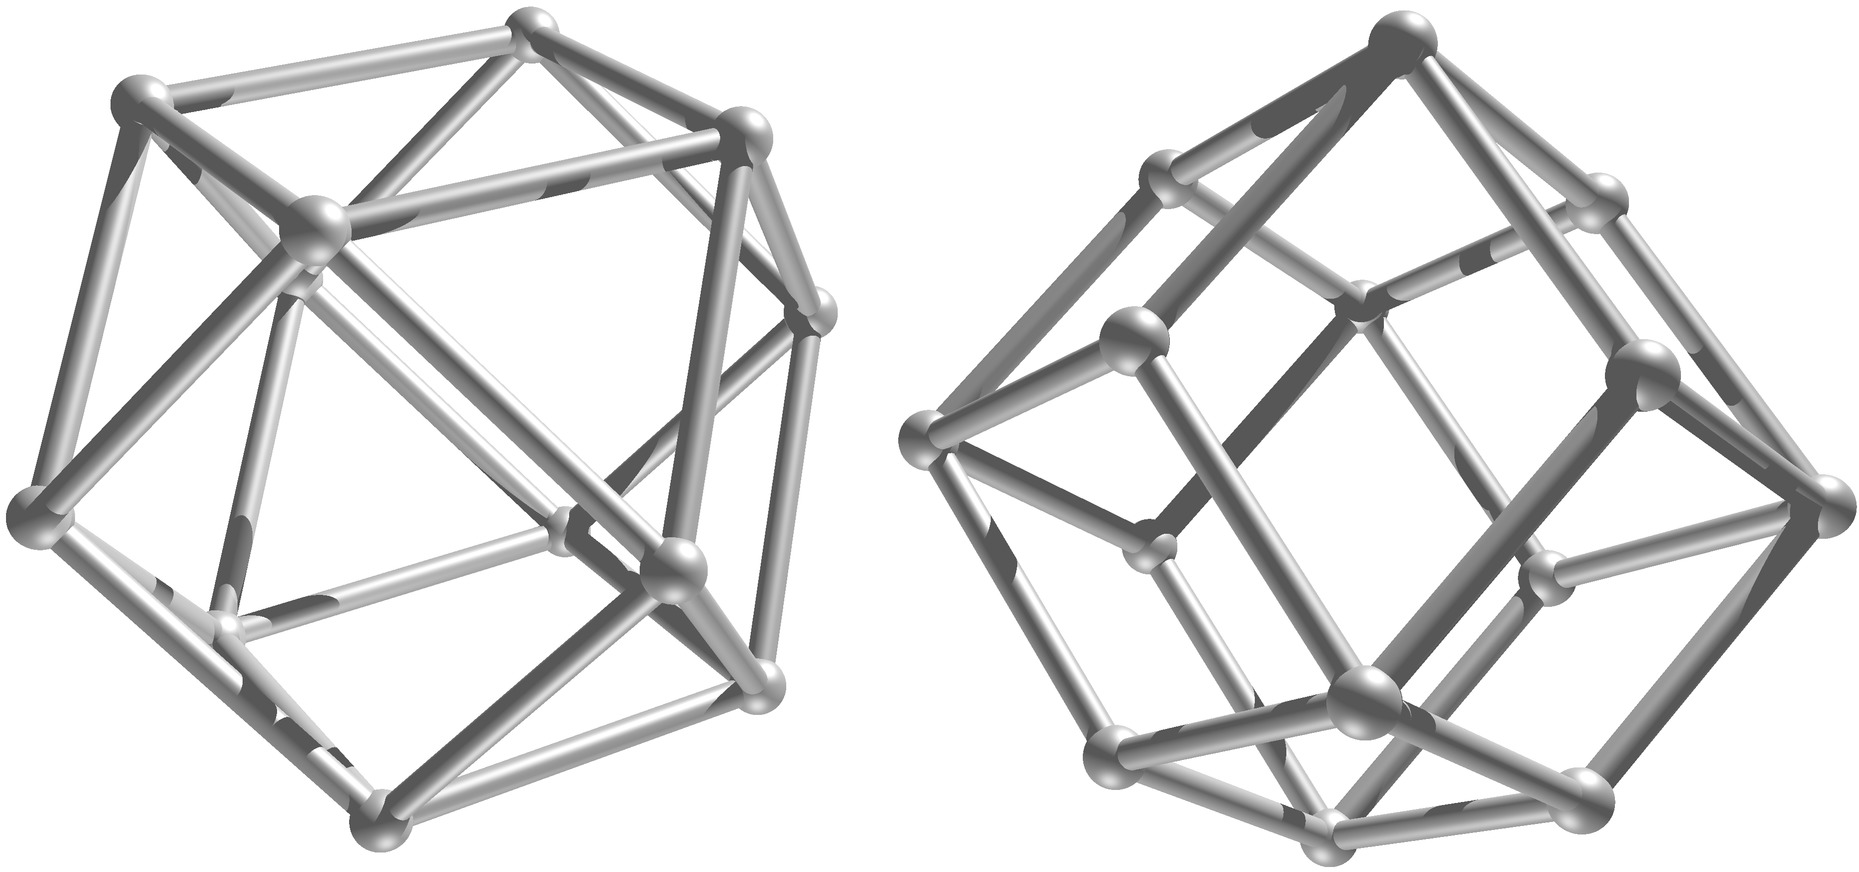
\includegraphics[width=\hsize]{kubooktaeder.jpg}
\caption{Kantennetzwerk von Kubooktaeder (links) und Rhombendodekaeder (rechts)
\label{kantennetzwerke}}
\end{figure}
\begin{figure}
\centering
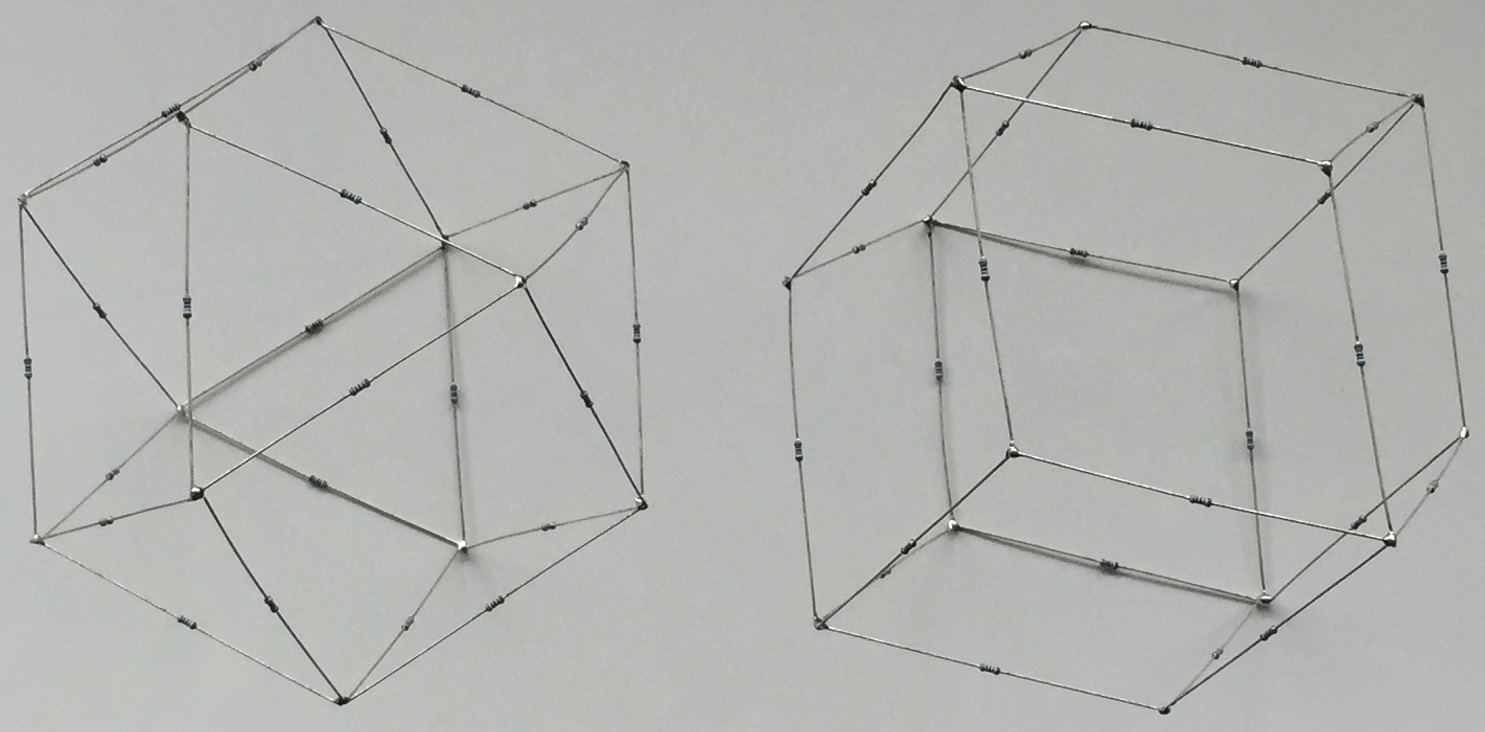
\includegraphics[width=\hsize]{realization.jpg}
\caption{Realisierung des Kantennetzwerks von Kuboktaeder (links)
und Rhombendodekaeder (rechts) mit 1k$\Omega$-Widerst"anden.
\label{realization}}
\end{figure}
Schneidet man einem W"urfel die Ecken durch Ebenen ab, die durch die
Kantenmitten gehen, erh"alt man ein neues Polyeder aus sechs Quadraten
und acht gleichseitigen Dreiecken, ein sogenanntes Kubooktaeder
(Abbildung~\ref{kantennetzwerke}, links).
Es besteht aus acht gleichseitigen Dreiecken und sechs Quadraten.
Den gleichen K"orper k"onnte man auch erhalten, indem man einem Oktaeder
die Ecken durch Ebenen durch die Kantenmitten abschneidet,
was den Namen plausibel macht.
Der dazu duale K"orper ist das Rhombendodekaeder, es besteht aus zw"olf Rhomben.

Die Dualit"at von Kubooktaeder und Rhombendodekaeder spiegelt sich auch in
den Symmetrieeigenschaften der Ecken und Seitenfl"achen.
Beim Kubooktader treffen in allen Ecken vier Kanten zusammen, aber in
verschiedenen Winkeln ($60^\circ$ und $90^\circ$).
Beim Kubooktaeder gibt es also nur eine Art von Ecken, aber zwei Arten von
Seitenfl"achen.
Beim Rhombendodekaeder dagegen gibt es nur eine Art von Seitenfl"achen,
aber zwei verschiedene Arten von Ecken, in denen drei oder vier
Kanten zusammentreffen.
Sie entsprechen nat"urlich den zwei verschiedenen Seitenfl"achen des 
Kubooktaeders.

Man kann das Rhombendodekaeder "ubrigens nicht dadurch erhalten, dass man
einfach die Seitenmitten des Kubooktaeders miteinander verbindet, denn die
Mitten der quadratischen Seitenfl"achen des Kubooktaeders liegen in der
gleichen Ebene wie zwei der Kanten der Dreiecksfl"achen.
Dies kann man auch in Abbildung~\ref{kantennetzwerke} sehr sch"on sehen.

Umgekehrt ist das Kubooktaeder tats"achlich dadurch realisierbar, dass
man die Seitenmitten des Rhombendodekaeders verbindet, was zum Beispiel
daraus folgt, dass man beim Rhombendodekaeder in jeder $n$-z"ahligen
Ecke (Ecke mit $n$ Kanten) auch eine $n$-fache Rotationssymmetrie hat,
w"ahrend beim Kubooktaeder in den 4-z"ahligen Ecken zwei Quadrate
und zwei Dreiecke zusammenkommen, so dass dort nur eine
$180^\circ$-Rotationssymmetrie m"oglich ist.

\section{Aufgabenstellung}

\newtheorem{aufgabe}{Aufgabe}
\begin{aufgabe}
Man berechne die "Aquivalentwiderst"ande "uber eine Kante eines mit
1k$\Omega$-Widerst"anden realisierten Kubookateders und eines
Rhombendodekaeders.
\end{aufgabe}

{\parindent0pt \bf Wettbewerbsbedingungen:}
\begin{enumerate}
\item
Die L"osung muss so dokumentiert sein, dass sie ohne weitere Hilfsmittel
nachvollziehbar ist.
\item
Es ist zul"assig, ein Computerprogramm zu verwenden, welches aber ebenfalls
soweit dokumentiert sein muss, dass man es nicht selbst kompilieren oder
ausf"uhren muss um zu verstehen, wie es funktioniert.
\item
Zur Kontrolle der eigenen L"osung stehen die Realisationen der beiden
Netzwerke zum Nachmessen zur Verf"ugung (Abbildung~\ref{realization}).
\item
Eingabefrist: 1.~November 2015, 00:00 Uhr.
\item
"Uber den Wettbewerb wird keine Korrespondenz gef"uhrt.
\end{enumerate}

\section{L"osung}
Die Theorie zur L"osung der vorliegenden Art von Problemen ist
im wesentlichen im Skript erkl"art, in der Vorlesung haben wir
uns vor allem auf das Aufstellen der Kirchhoff-Gleichungen 
konzentriert.
Damit man den Widerstand bestimmen kann, muss man irgendwie eine
Spannungsquelle anschliessen und die entstehende Spannungs- und Stromverteilung
berechnen.
Dies ist auf verschiedene Arten m"oglich, und ist in Abschnitt~\ref{quelle}
diskutiert.

Beide Netzwerke haben 24 Kanten, f"ur die L"osung m"ussen also etwas
unhandliche Gleichungssysteme gel"ost werden.
Abschnitt~\ref{vereinfachung} beschreibt, wie man die Netzwerke und
damit die Gleichungssysteme vereinfachen kann.

Das im Skript beschriebene L"osungsverfahren verlangt zun"achst,
dass die Matrix $\partial$ der Verbindungen im Netzwerk aufgestellt
wird, sie ergibt dann bereits die Knotengleichung $\partial I=0$.
Aus $\partial$ kann eine minimale Menge von Maschen gewonnen werden,
die die Spalten der Matrix $Z$ bilden.
Die Maschengleichungen sind dann
\[
Z^tRI=Z^te,
\]
wobei $e$ der Vektor der Spannungen in den Kanten ist.
Da die Zeilen von $\partial$ linear abh"angig sind, kann man
einfach die letzte Zeile weglassen, so dass zusammen mit der Matrix $Z^tI$
eine regul"are quadratische $n\times n$-Matrix entsteht.

F"ur dieses spezielle Netzwerk kann man jedoch die Kirchhoff-Gleichungen
auch noch auf andere Art bekommen.
Da das Netzwerk das Kantennetzwerk eines Polyeders ist, kann man als
Maschen genau die R"ander der Seitenfl"achen des Polyeders verwenden.
Man nennt dies auch die Kreisstrommethode.

\subsection{Spannungsquellen\label{quelle}}
Um den "Aquivalentwiderstand "uber eine Kante zu ermitteln, muss
eine Spannungsquelle hinzugef"ugt werden, die im Netzwerk einen
Strom hervorruft.
Wir nehmen im folgenden an, dass der Widerstand zwischen den Knoten
$1$ und $2$ ermittelt werden soll.

Man kann zum Beispiel in den Knotengleichungen $\partial I=0$
die rechte Seite modifizieren.
In der ersten Knotengleichung setzt man die rechte Seite auf $i_0$,
in der zweiten auf $-i_0$.
Die L"osung des Gleichungssystems liefert dann den die Spannung $u_0$ zwischen
den beiden Knoten $1$ und $2$, und damit kann der "Aquivalent-Widerstand
als $u_0/i_0$ berechnet werden.

Die zweite M"oglichkeit ist, dass man dem Netzwerk eine zus"atzliche
Kante hinzuf"ugt, die eine Spannungsquelle enth"alt. 
Das Gleichungssystem wird dadurch etwas gr"osser, man kann zum
Beispiel die Masche bestehend aus der interessierenden Kante und
der Spannungsquelle hinzuf"ugen.
Ist $i_0$ der Strom in dieser Masche und $u_0$ die Spannung der
Spannungsquelle, dann kann man den Widerstand wieder als $u_0/i_0$
finden.

\begin{figure}
\centering
\includestandalone{spannungsquelle}
\caption{Ersetzung des Widerstands $R_{jk}$ (links)
zwischen den Knoten $j$ und $k$
des Netzwerkes durch eine Spannungsquelle mit Spannung $u_{jk}$ (rechts),
$R'$ ist der Widerstand des Netzwerkes ohne die Kante $R_{jk}$.
\label{spannungsquelle}}
\end{figure}
Die geringsten Modifikationen am Gleichungssystem sind n"otig, wenn
man die Spannungsquelle mit mit Spannung $u_{jk}$ in die interessierende
Kante vom Knoten $j$ zum Knoten $k$ einbaut.
Das Netzwerk k"onnen wir vereinfachen zu einem Netzwerk bestehend
aus nur zwei Widerst"anden, n"amlich dem Widerstand $R_{jk}$ der Kante zwischen
den Knoten $j$ und $k$, und dem Widerstand $R'$ des restlichen Netzwerkes.
Wir k"onnen dann den Widerstand der Kante durch eine Spannungsquelle
$u_{jk}$ ersetzen (Abbildung~\ref{spannungsquelle}). 
Der durch den Widerstand $R'$ fliessende Strom $I'$ kann aus den
Kirchhoff-Gleichungen berechnet werden, und damit
auch der Widerstand $R'=u_{jk}/I'$.
Der gesuchte Widerstand $r$ des Gesamtnetzwerkes ist die Parallelschaltung
von $R_{jk}$ und $R'$, also
\[
\frac1r=\frac1{R_{jk}}+\frac{I'}{u_{jk}}.
\]

\subsection{Resultate}
Die Durchf"uhrung der Rechnung ergibt:
\begin{align*}
R_{\text{Kubooktaeder}}
&=
458.3333\Omega
\\
R_{\text{Rhombendodekaeder}}
&=
541.6666\Omega
\end{align*}
Man stellt fest, dass die Summe der Widerst"ande 1k$\Omega$ ist, 
eine Eigenschaft, die sich auf duale Kanten in beliebigen dualen
Netzwerken verallgemeinern l"asst.

\subsection{Vereinfachungen\label{vereinfachung}}
Die Gleichungssystem zur Berechnung des Widerstandes sind ziemlich gross,
immerhin haben beide Netzwerke 24 Kanten und damit mindestens im Prinzip 
24 unbekannte Str"ome oder Spannungen, die zu bestimmen sind.
\begin{figure}
\centering
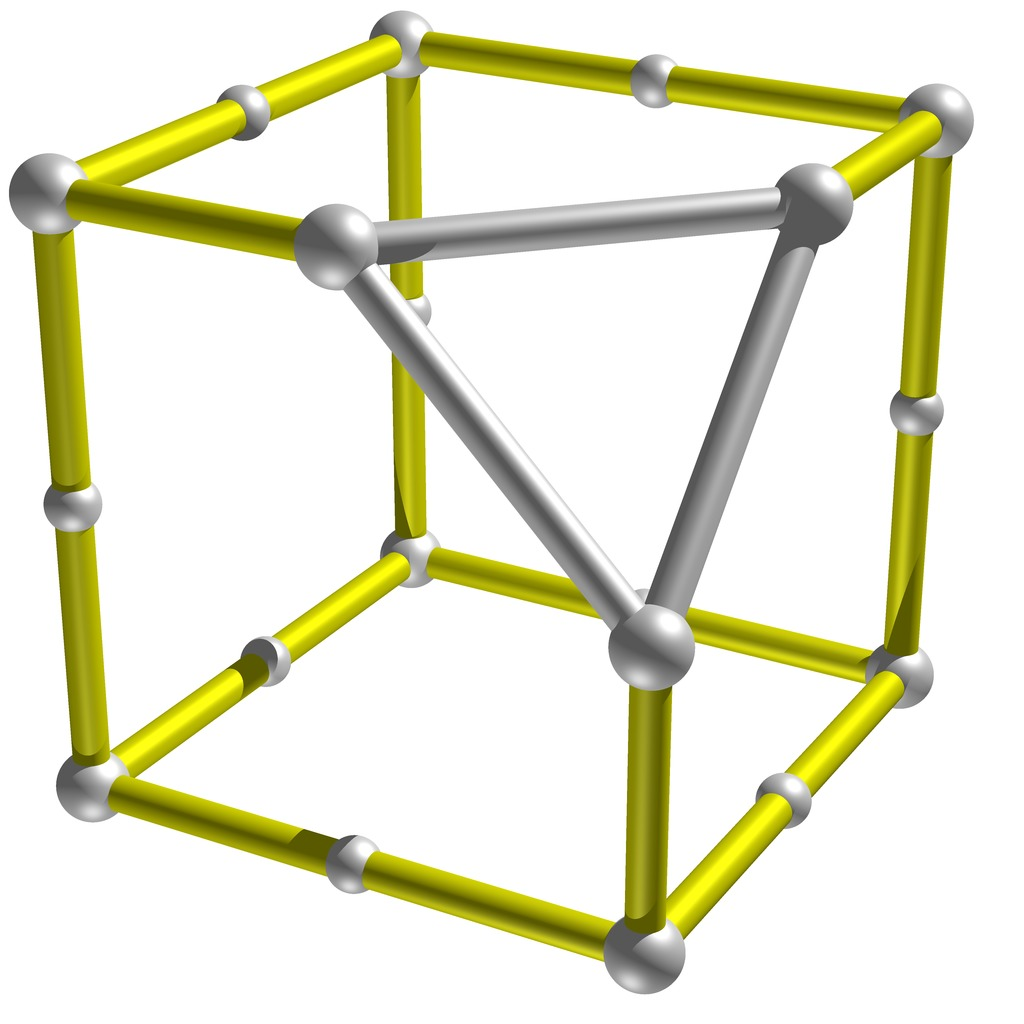
\includegraphics[width=0.45\hsize]{vereinfachung.jpg}
\quad
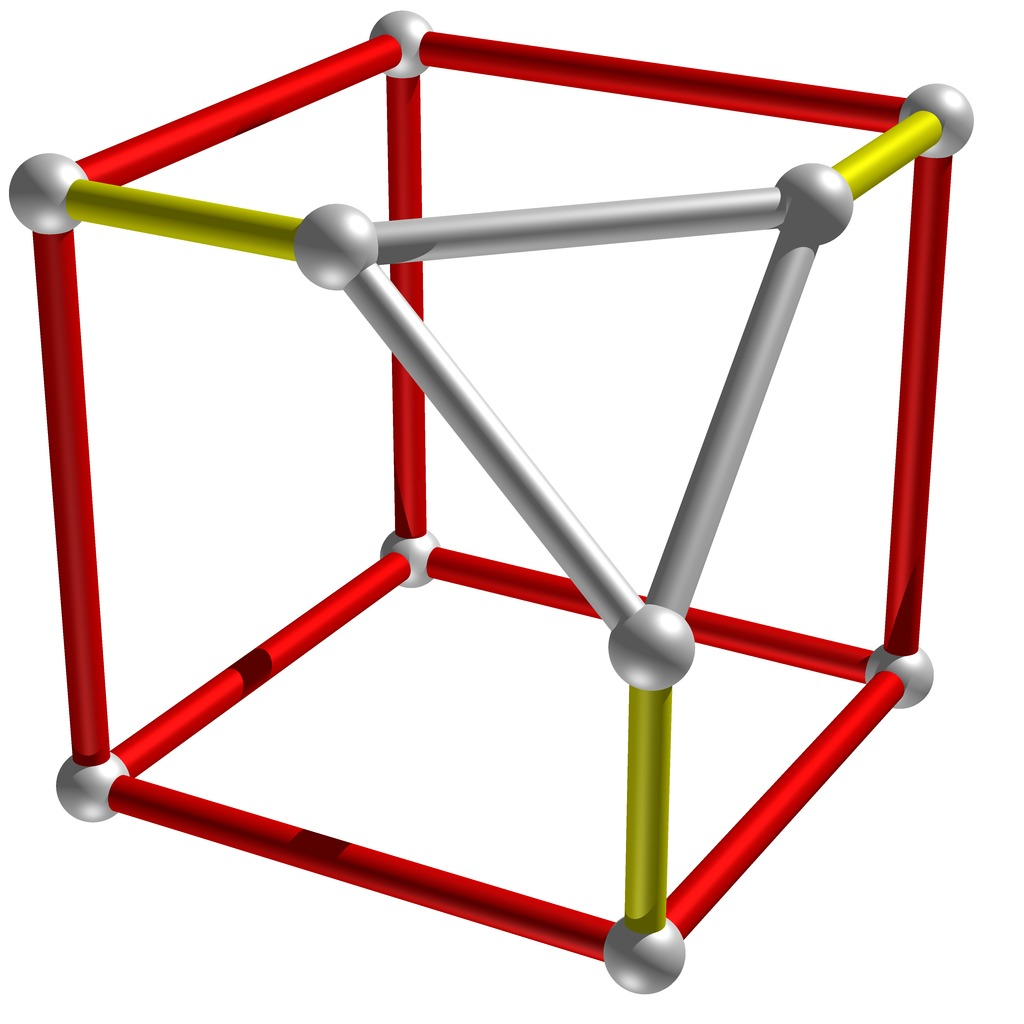
\includegraphics[width=0.45\hsize]{vereinfachung2.jpg}
\caption{Vereinfachung des Kubooktaeders mit Hilfe der Stern-Dreieck-Methode.
F"unf Dreiecke werden durch die gelben Sterne ersetzt (links),
danach k"onnen zwei gelbe Kanten in Serie durch eine rote Kante
ersetzt werden (rechts).
\label{wuerfel}}
\end{figure}
\begin{figure}
\centering
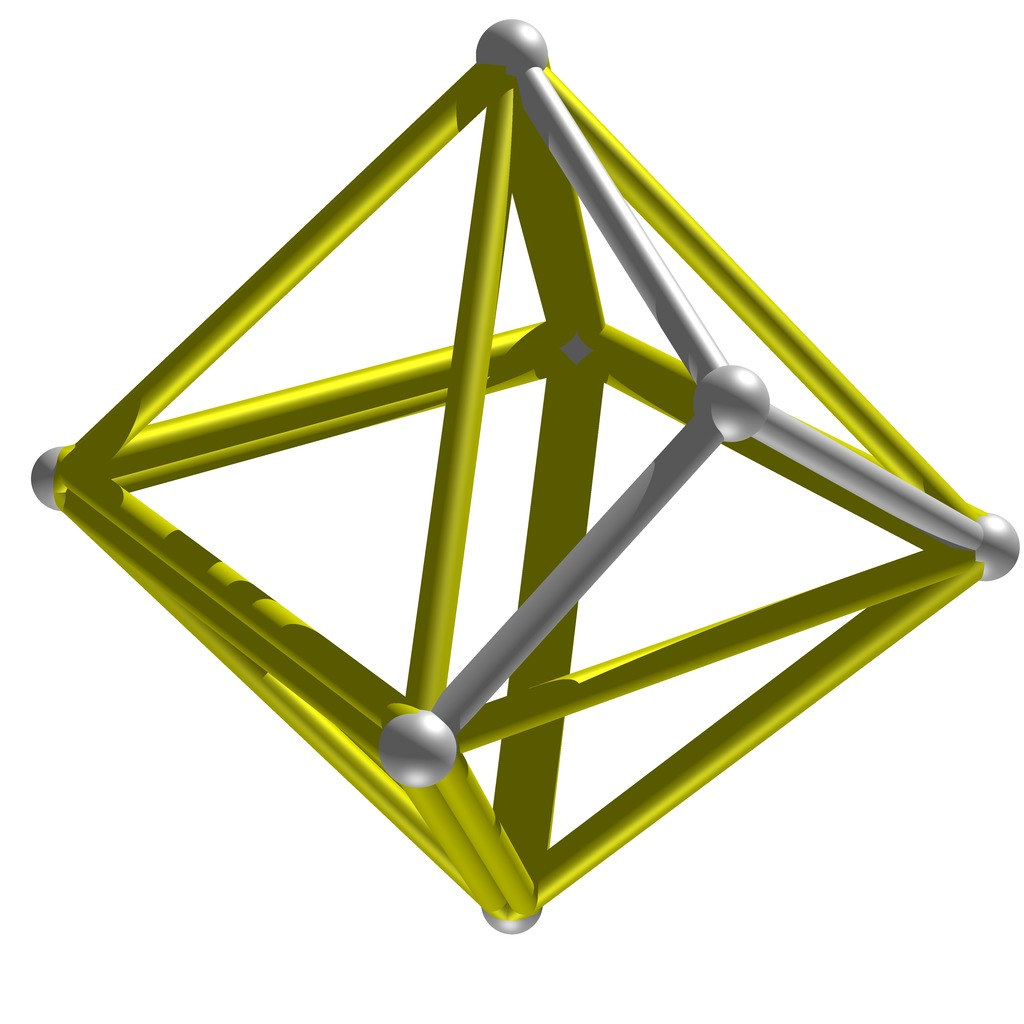
\includegraphics[width=0.45\hsize]{oktaeder.jpg}
\quad
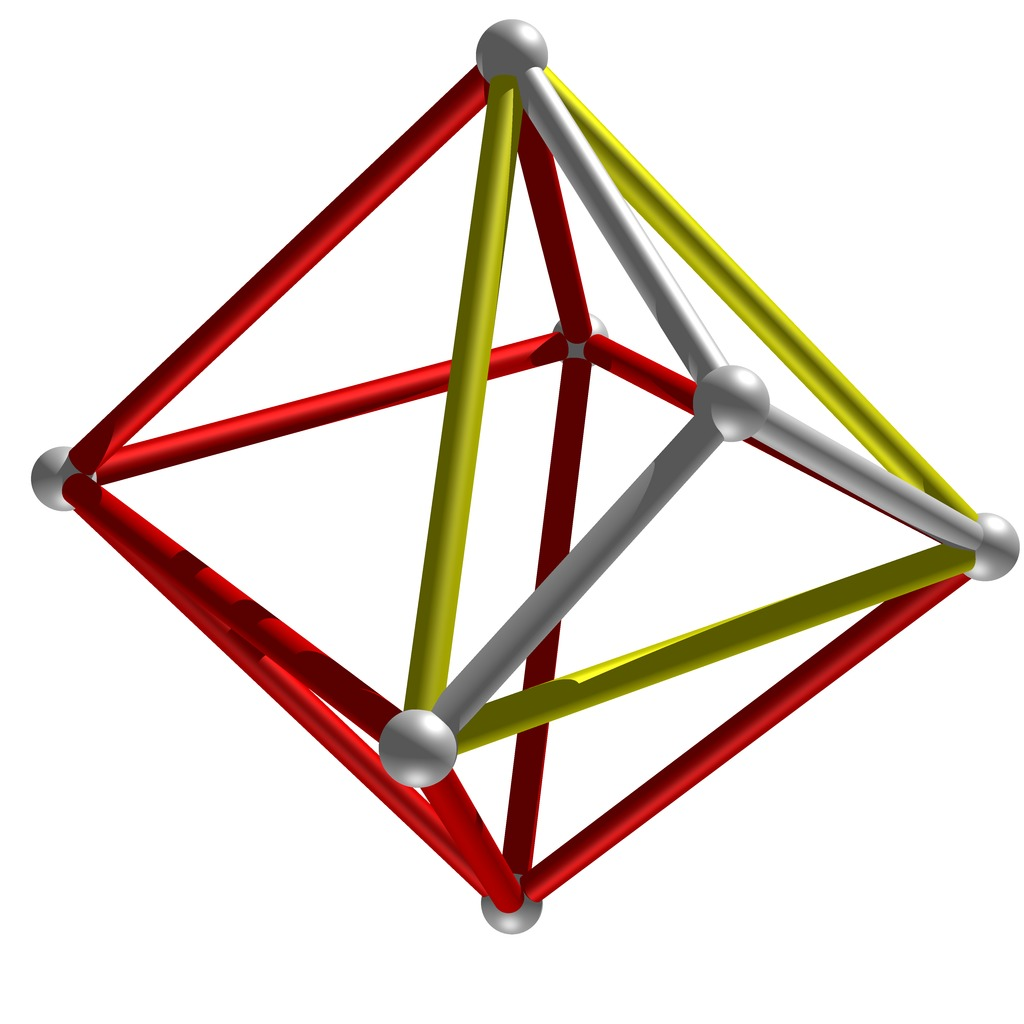
\includegraphics[width=0.45\hsize]{oktaeder2.jpg}
\caption{Vereinfachung des Rhombendodekaeders mit Hilfe der
Stern-Dreieck-Methode.
F"unf Sterne werden ersetzt durch die gelben Dreiecke (links), und
anschliessend die parallelen Kanten zu einer roten Kante zusammengefasst
(rechts).
\label{oktaeder}}
\end{figure}
Ersetzt man im Kubooktaeder jedes Dreieck durch einen Stern
wird daraus ein W"urfel.
Ebenso wird aus dem Rhombendodekaeder ein Oktaeder, wenn man
jeden Stern durch ein Dreieck ersetzt.
W"urfel und Oktaeder sind ebenfalls dual zueinander, haben aber 
nur zw"olf Kanten und acht bzw.~sechs Ecken, die Gleichungen
f"ur diese beiden Netzwerke w"aren also deutlich einfacher.
Ausserdem bleibt die Eigenschaft erhalten, dass alle Widerst"ande
gleich gross sind.

Allerdings bringen diese Transformationen auch die Kante zum
verschwinden, "uber die der "Aquivalent-Widerstand bestimmt werden
soll.
Die Transformation muss daher im Falle des Kubooktaeders ein Dreieck 
und im Falle des Rhombendodekaeders einen Stern unber"uhrt lassen.
Wie die Abbildungen \ref{wuerfel}{} und \ref{oktaeder}
zeigen, werden im resultierenden Netzwerk drei verschiedene Widerstandswerte
auftreten.

Nadja Rutz hat in ihrer L"osung beide Netzwerke in der oben genannten
Art verwendet, w"ahrend Matthias Schneider die Transformation nur beim
Kubooktaeder durchgef"uhrt hat.

Die Vereinfachungen k"onnten aber noch weiter getrieben werden.
Die Ersetzung eines Sterns durch ein Dreieck ist in Abbildung~\ref{stern3}
dargestellt.

\begin{figure}
\centering
\includestandalone{stern}
\caption{Stern-Dreieck-Ersetzung
\label{stern3}}
\end{figure}
Die Ersetzung eines Sterns durch ein Dreieck ist auch f"ur $n$-Ecke
m"oglich, mindestens f"ur ungerade $n$.
F"ur gerade $n$ sind zus"atzliche Bedingungen n"otig.
Man kann die Gleichungen f"ur die Widerst"ande $R_i$ ablesen:
\begin{equation}
\begin{linsys}{3}
R_1&+&R_2& &   &=&\displaystyle\biggl(\frac1{r_1}+\frac1{s-r_1}\biggr)^{-1}\\
   & &R_2&+&R_3&=&\displaystyle\biggl(\frac1{r_2}+\frac1{s-r_2}\biggr)^{-1}\\
R_1& &   &+&R_3&=&\displaystyle\biggl(\frac1{r_3}+\frac1{s-r_3}\biggr)^{-1}
\end{linsys}
\label{dreieck}
\end{equation}
mit $s=r_1+r_2+r_3$.
Es ist wohlbekannt, dass das Gleichungsystem die L"osung
\[
R_i=\frac{r_1r_2r_3}{s}\cdot\frac1{r_i}
\]
hat.

Eine analoge Ersetzung ist auch m"oglich f"ur ein $n$-Eck.
Die Gleichungen, die (\ref{dreieck}) entsprechen, werden dabei zu
\begin{equation}
\begin{linsys}{6}
R_1&+&R_2& &   & &   & &   & &   &=&
	\displaystyle\biggl(\frac1{r_1}+\frac1{s-r_1}\biggr)^{-1}\\
   & &R_2&+&R_3& &   & &   & &   &=&
	\displaystyle\biggl(\frac1{r_2}+\frac1{s-r_2}\biggr)^{-1}\\
   & &   & &R_3&+&R_4& &   & &   &=&
	\displaystyle\biggl(\frac1{r_3}+\frac1{s-r_3}\biggr)^{-1}\\
   & &   & &   & &\ddots& &\ddots& &   & &\\
R_1& &   & &   & &   & &   &+&R_n&=&
	\displaystyle\biggl(\frac1{r_n}+\frac1{s-r_n}\biggr)^{-1}
\end{linsys}
\label{nstern}
\end{equation}
Die linke Seite kann als lineares Gleichungssystem mit der Koeffizientenmatrix
\[
A_n=\begin{pmatrix}
     1&     1&     0& \dots&     0&     0\\
     0&     1&     1& \dots&     0&     0\\
     0&     0&     1& \dots&     0&     0\\
\vdots&\vdots&\vdots&\ddots&\vdots&\vdots\\
     0&     0&     0& \dots&     1&     1\\
     1&     0&     0& \dots&     0&     1
\end{pmatrix}
\]
geschrieben werden.
Die $n\times n$-Matrix $A_n$ ist nur f"ur ungerade $n$ invertierbar.
Man kann n"amlich die Determinante mit Hilfe des Entwicklungssatzes berechnen:
\begin{align*}
\det(A_n)
&=
\left|
\begin{matrix}
     1&     1& \dots&     0&     0\\
     0&     1& \dots&     0&     0\\
\vdots&\vdots&\ddots&\vdots&\vdots\\
     0&     0& \dots&     1&     1\\
     0&     0& \dots&     0&     1
\end{matrix}
\right|
-(-1)^n
\left|
\begin{matrix}
     1&     0& \dots&     0&     0\\
     1&     1& \dots&     0&     0\\
     0&     1& \dots&     0&     0\\
\vdots&\vdots&\ddots&\vdots&\vdots\\
     0&     0& \dots&     1&     1
\end{matrix}
\right|
=1-(-1)^n
=\begin{cases}
2&\quad\text{$n$ ungerade}\\
0&\quad\text{$n$ gerade}
\end{cases}
\end{align*}
F"ur ungerade $n$ ist also die Ersetzung eines $n$-Sterns durch ein $n$-Eck
oder umgekehrt immer auf eindeutige Art m"oglich.

F"ur gerade $n$ ist die Matrix $A_n$ nicht invertierbar, damit die
Gleichungen (\ref{nstern}) l"osbar sind, m"ussen die rechten Seiten eine
zus"atzliche lineare Bedingung erf"ullen.
Nehmen wir an, dass die Bedingung die Form
\[
\sum_{i=1}^nb_i\biggl(\frac1{r_i}+\frac1{s-r_i}\biggr)^{-1}=0
\]
mit Koeffizienten $b_i$ hat.
Da $A_n$ nicht regul"ar ist, m"ussen alle Spalten von $A_n$ die
Bedingung erf"ullen, es muss also gelten
\[
A^tb=0\qquad \text{mit}\;
b=\begin{pmatrix}b_1\\\vdots\\b_n\end{pmatrix}.
\]
Das Gleichungssystem  kann mit dem Gaussalgorithmus gel"ost werden:
\begin{align*}
\begin{tabular}{|
>{$}c<{$}
>{$}c<{$}
>{$}c<{$}
>{$}c<{$}
>{$}c<{$}
>{$}c<{$}
>{$}r<{$}
|}
\hline
     1&     0&     0&     0& \dots&     0&     1\\
     1&     1&     0&     0& \dots&     0&     0\\
     0&     1&     1&     0& \dots&     0&     0\\
     0&     0&     1&     1& \dots&     0&     0\\
\vdots&\vdots&\vdots&\vdots&\ddots& \dots&\vdots\\
     0&     0&     0&     0& \dots&     1&     0\\
     0&     0&     0&     0& \dots&     1&     1\\
\hline
\end{tabular}
&\rightarrow
\dots
\rightarrow
\begin{tabular}{|
>{$}c<{$}
>{$}c<{$}
>{$}c<{$}
>{$}c<{$}
>{$}c<{$}
>{$}c<{$}
>{$}r<{$}
|}
\hline
     1&     0&     0&     0& \dots&     0&     1\\
     0&     1&     0&     0& \dots&     0&    -1\\
     0&     0&     1&     0& \dots&     0&     1\\
     0&     0&     0&     1& \dots&     0&    -1\\
\vdots&\vdots&\vdots&\vdots&\ddots&\ddots&\vdots\\
     0&     0&     0&     0& \dots&     1&     1\\
     0&     0&     0&     0& \dots&     0&     0\\
\hline
\end{tabular}
\end{align*}
Man kann ablesen, dass $\operatorname{Rang}A_n=n-1$ ist, und dass f"ur
die $b_i$ die Zahlen $b_i=(-1)^i$ eine L"osung sind.
Das Gleichungssystem (\ref{nstern})  ist
genau dann l"osbar , wenn die rechten Seiten die Bedinung
\begin{equation}
\sum_{i=1}^n (-1)^i \biggl(\frac1{r_i}+\frac1{s-r_i}\biggr)^{-1}=0
\label{condition}
\end{equation}
erf"ullt ist.
Sie ist insbesondere dann erf"ullt, wenn die Widerst"ande $r_i$
alle gleich sind.
%Durch "Ubergang zu Leitf"ahigkeiten k"onnen analoge Gleichungen f"ur
%die Ersetzung in der umgekehrten Richtung formuliert werden.

Im Falle des Rhombendodekaeders, das zum gr"ossten Teil bereits in
ein Oktaeder umgewandelt wurde wie in Abbildung~\ref{oktaeder},
sind zwei 4-Sterne aus identischen Widerst"anden vorhanden.
Ein $n$-Stern aus identischen Widerst"anden $R$ kann durch ein $n$-Eck
aus ebenfalls identischen Widerst"anden $r$ ersetzt werden, und es
gilt
\begin{align*}
\frac{1}{2R}
&=
\frac{1}{r}+\frac{1}{(n-1)r}
\\
\frac{1}{2R}
&=
\frac{1}{r}
\biggl(1+\frac1{n-1}\biggr)
=
\frac{1}{r}\frac{n}{n-1}
\\
r&=\frac{2nR}{n-1}.
\end{align*}
Damit l"asst sich der 4-Stern ebenfalls eliminieren.

Durch Anwendung dieser Ersetzungen kann das Netzwerk sukzessive 
vereinfacht werden bis nur noch die Verbindung zwischen den zwei
ausgew"ahlten Ecken "ubrig bleibt.

\subsection{Vermutungen}
Matthias Schneider hat aufgrund der numerischen Resultate vermutet,
dass der Widerstand sich direkt aus der Anzahl $E$ der Ecken und
und der Anzahl $K$ der Kanten ermitteln l"asst:
\[
R=\frac{E-1}{K}.
\]
So eine Formel kann nat"urlich nur zutreffen, wenn alle Kanten
des Netzwerks gleichwertig sind. 
Die vorliegenden Netzwerke erf"ullen diese Bedingung, aber
auch die Kanten der platonischen K"orper (regelm"assigen Polyeder),
und die Vermutung trifft auch dort zu.

Kubooktaeder und Rhombendodekaeder sind zueinander dual.
Bezeichnen wir die Fl"achen\-, Kanten- und Ecken-Zahl des
Kubooktaeders mit $F_1$, $K_1$ und $E_1$ und die entsprechenden
Zahlen des Rhombendodekaeders mit $F_2$, $K_2$ und $E_2$, dann
bedeutet die Dualit"at, dass gilt
\begin{equation}
\begin{aligned}
F_1&=E_2,&\qquad
K_1&=K_2,&\qquad
E_1&=F_2.
\end{aligned}
\label{dualitaet}
\end{equation}
Der Eulersche Polyeder-Satz besagt, dass f"ur die Zahlen $F$, $K$ und $E$
jedes Polyeders die Beziehung
\begin{equation}
E-K+F=2
\qquad
\Rightarrow
\qquad
E+F-2=K
\label{euler}
\end{equation}
gilt.
Die Widerst"ande sind gem"ass obiger Vermutung $R_i=(E_i-1)/K_i$.
und deren Summe wird unter Verwendung von (\ref{dualitaet}) 
und (\ref{euler})
\begin{align*}
R_1+R_2
&=
\frac{E_1-1}{K_1}
+
\frac{E_2-1}{K_2}
=
\frac{E_1+F_1-2}{K_1}
=
\frac{K_1}{K_1}=1.
\end{align*}
Auch diese Beziehung kann nat"urlich nur gelten, wenn alle Kanten den
gleichen Widerstand haben.

Bei dualen Netzwerk k"onnen wir zu jeder Kante im einen Netzwerk die dazu
geh"orige duale Kante im dualen Netzwerk identifizieren.
Selbst wenn die Widerst"ande der Kanten verschieden sind, kann man
eine einfache Beziehung zwischen den "Aquivalentwiderst"anden zueinander
dualer Kanten beweisen.

\subsection{Widerstands-Distanz}
Man kann aus den Kirchhoff-Gleichungen f"ur die Str"ome unter Verwendung
des ohmschen Gesetzes auch eine Gleichung f"ur die Spannungen herleiten.
Da die Maschengleichungen nur Ausdruck des ohmschen Gesetzes sind, kann
man das Problem nun ausschliesslich mit den Knotengleichungen l"osen.
Man erh"alt so das Konzept der Widerstandsdistanz in einem Graphen,
welches im Folgenden entwickelt werden soll.

\subsubsection{Laplace-Operator}
Sei $U$ der Vektor der Potentiale in den Knoten.
Wenn es eine Kante zwischen den Knoten $j$ und $k$ gibt, dann gibt es
auch eine Spalte in $\partial$, die in der Position $j$ eine $-1$ und
in der Position $k$ eine $1$ (oder umgekehrt) enth"alt.
Die Potential-Differenz $U_k-U_j$ l"asst sich also bestimmen, indem
man $U$  mit dieser Zeile multipliziert.
Die Potentialdifferenzen entlang der Kanten sind also
$\partial^tU$.

Das ohmsche Gesetz stellt den Zusammenhang zwischen Spannungsdifferenzen
und Str"omen her, es gilt
\[
U=RI
\qquad
\Rightarrow
\qquad
I=R^{-1}\partial^t U.
\]
Schreibt man $S=R^{-1}$ f"ur die Leitwertmatrix, wie dies auch im Skript
gemacht wird, dann werden 
die Knotengleichungen $\partial I=0$ zu
\begin{equation}
\partial I=\partial S\partial^t U=0.
\label{stromgleichung}
\end{equation}
Die Matrix $\Delta=\partial S\partial^t$ heisst der Laplace-Operator des
Netzwerks.
Da $\Delta$ nur soviele Zeilen und Spalten hat, wie das Netzwerk
Knoten hat, sind diese Gleichungen viel einfacher, also die vollen
Kirchhoff-Gleichungen, die soviele Zeilen und Spalten haben wie
das Netzwerk Kanten hat.

In unserem Fall sind alle Widerst"ande und damit auch alle Leitwerte
gleich, man braucht nur noch die Matrix $\Delta=\partial\partial^t$ zu
bestimmen.
Die Matrix $\Delta$ l"asst sich wie $\partial$ direkt aus der Geometrie
des Netzwerkes ablesen.
Auf der Diagonalen steht die Anzahl der Verbindungen, die von einem
Knoten ausgehen, und in der Zeile und Spalte eines Knotens steht
f"ur jede Verbindung zu einem anderen Knoten ein $-1$.

\begin{figure}
\centering
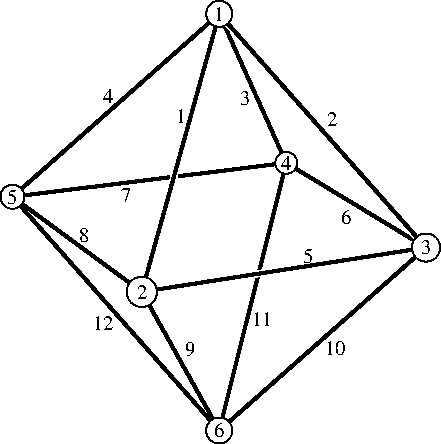
\includegraphics{../aufgaben/1/10000028/octahedron-1.pdf}
\caption{Oktaeder mit numerierten Ecken und Kanten
\label{oktaeder-kanten}}
\end{figure}
Da die Matrizen $\partial$ f"ur Kubooktaeder und Rhombendodekaeder
sehr umfangreich sind, bestimmen wir als Beispiele f"ur das Gesagte
die entsprechenden Matrizen f"ur ein Oktaeder wie in
Abbildung~\ref{oktaeder-kanten}.
Der Operator $\partial$ ist
\[
\setcounter{MaxMatrixCols}{20}
\partial=\begin{pmatrix}
%1   2  3  4  5  6  7  8  9 10 11 12
-1& -1&-1&-1& 0& 0& 0& 0& 0& 0& 0& 0\\ %  1
 1&  0& 0& 0&-1& 0& 0&-1&-1& 0& 0& 0\\ %  2
 0&  1& 0& 0& 1&-1& 0& 0& 0&-1& 0& 0\\ %  3
 0&  0& 1& 0& 0& 1&-1& 0& 0& 0&-1& 0\\ %  4
 0&  0& 0& 1& 0& 0& 1& 1& 0& 0& 0&-1\\ %  5
 0&  0& 0& 0& 0& 0& 0& 0& 1& 1& 1& 1   %  6
\end{pmatrix}
\]
Der zugeh"orige Laplace-Operator ist
\[
\Delta=\partial\partial^t
=\begin{pmatrix}
%  1   2   3   4   5   6
   4& -1& -1& -1& -1&  0\\
  -1&  4& -1&  0& -1& -1\\
  -1& -1&  4& -1&  0& -1\\
  -1&  0& -1&  4& -1& -1\\
  -1& -1&  0& -1&  4& -1\\
   0& -1& -1& -1& -1&  4
\end{pmatrix}.
\]
Statt mit $6\times 12$-Matrix  $\partial$ muss man jetzt nur noch
die halb so grosse $6\times 6$-Matrix $\Delta$ studieren.

\subsubsection{Potentialgleichung}
Um mit $\Delta$ den "Aquivalentwiderstand "uber die Kanten zwischen den
Knoten $j$ und $k$ zu bestimmen, muss man am Knoten $j$ einen
Strom $i_0$ einspeisen und beim Knoten $k$ wieder entnehmen.
Die sich einstellende Potentialdifferenz $U_j-U_k$ ist proportional
zum gesuchten Widerstand.
Die Knotengleichungen (\ref{stromgleichung}) werden durch das Einspeisen
des Stromes modifiziert, die rechte Seite ist nicht mehr $0$, sondern
enth"alt an der Stelle $j$ den Strom $i_0$ und ander Stelle $k$ den
Strom $-i_0$.
Es ist also die Gleichung
\begin{equation}
\Delta U=
\begin{pmatrix}\vdots\\i_0\\\vdots\\-i_0\\\vdots\end{pmatrix}
=i
\label{distanzgleichung}
\end{equation}
zu l"osen.

W"are $\Delta$ invertierbar, und w"are $\Omega$ mit den Matrixelementen
$\Omega_{jk}$ die Inverse von $\Delta$,
dann k"onnte man die interessierenden Potentiale $U_j$ und $U_k$
einfach aus dem Produkt $\Omega i$ finden:
\[
\begin{pmatrix}
\vdots\\
U_j\\
\vdots\\
U_k\\
\vdots
\end{pmatrix}
=
\Omega i
=
\Omega
\begin{pmatrix}\vdots\\i_0\\\vdots\\-i_0\\\vdots\end{pmatrix}
=
\begin{pmatrix}
\vdots\\
\Omega_{jj}i_0-\Omega_{jk}i_0\\
\vdots\\
\Omega_{kj}i_0-\Omega_{kk}i_0\\
\vdots
\end{pmatrix}.
\]
Daraus kann man dann den Widerstand ablesen:
\begin{equation}
R_{jk}
=
\frac{U_j-U_k}{i_0}
=
\Omega_{jj}-\Omega_{jk}
-(\Omega_{kj}-\Omega_{kk})
=
\Omega_{jj}
+\Omega_{kk}
-\Omega_{jk}
-\Omega_{kj}.
\label{widerstandsdistanz}
\end{equation}
\newtheorem{definition}{Definition}
\begin{definition}
Der Widerstand
\[
R_{jk}
=
\Omega_{jj}
+\Omega_{kk}
-\Omega_{jk}
-\Omega_{kj}
\]
heisst die {\em Widerstandsdistanz} zwischen den Knoten $j$ und $k$.
\end{definition}

\subsubsection{L"osbarkeit\label{loesbarkeit}}
Leider ist die Matrix $\Delta$ nicht invertierbar.
Da eine Spalte genau so viele $-1$ enth"alt, wie der zugeh"orige Knoten
Verbindungen hat, summieren sich diese $-1$ mit der Anzahl der Verbindungen
auf der Diagonalen zu $0$.
Die Summe aller Zeilen von $\Delta$ ist also $0$.
Diese lineare Beziehung zwischen den Zeilen von $\Delta$ zeigt, dass 
$\Delta$ nicht vollen Rang hat.
Mit dem Vektor $a$ bestehend aus lauter Einsen kann
man diese Summeneigenschaft auch als
\begin{equation}
\Delta a
=
\Delta\begin{pmatrix}1\\1\\\vdots\\1\end{pmatrix}
=0
\end{equation}
schreiben.
Da $\Delta=\partial\partial^t$ symmetrisch ist\footnote{Man kann zum Beispiel
$\Delta^t=(\partial\partial^t)^t=(\partial^t)^t\partial^t=\partial\partial^t
=\Delta$ nachrechnen.}, muss auch $a^t\Delta=0$ gelten.
Insbesondere kann die die Gleichung $\Delta U=i$ nur dann eine L"osung
haben, wenn auch $i$ die Bedingung $a^ti=0$ erf"ullt.
F"ur die Str"ome in (\ref{distanzgleichung}) ist diese Bedingung
\[
a^ti=
\begin{pmatrix}1&1&\dots&1\end{pmatrix}\begin{pmatrix}1\\1\\\vdots\\1\end{pmatrix}
=i_0-i_0=0,
\]
also automatisch erf"ullt, die Gleichung wird eine L"osung haben.

Die L"osung der Gleichung $\Delta U=i$ ist nicht eindeutig.
Addiert man zu einer L"osung eine beliebige L"osung der homogenen Gleichung
$\Delta U=0$, dann ergibt sich wieder eine L"osung.
Die L"osung der homogenen Gleichung ist aber ein Vielfaches von $a$,
und addieren des gleichen Wertes in allen Elementen von $U$ ist physikalisch
nichts anderes als die Wahl eines anderen Potentialnullpunktes,
insbesondere hat sie auf die Berechnung der Potentialdifferenz zwischen
den Knoten $j$ und $k$ keinen Einfluss.

\subsubsection{Pseudoinverse}
Die Definition der Widerstandsdistanz beruhte auf der M"oglichkeit, eine
Inverse f"ur $\Delta$ zu finden, die aber nach Abschnitt~\ref{loesbarkeit}
gar nicht existieren kann.
Es wird also eine Konstruktion einer Matrix $\Omega$ gesucht, die
die Rolle der Inversen "ubernehmen kann.
Sie muss f"ur alle in Frage kommenden Vektoren $i$ eine L"osung $U$
der Gleichung $\Delta U=i$ liefern.
Dies wird erreicht, wenn $\Omega$ die Matrix $\Omega$ ist, die
$\Delta\Omega i=i$ liefert f"ur Vektoren, die die Bedingung  $a^ti=0$ erf"ullen.

Die sogenannte Pseudoinverse kann die Rolle von $\Omega$ "ubernehmen, ihre
allgemeine Definition ist jedoch erst mit der Singul"arwertzerlegung
m"oglich, die erst im Kapitel~5 des Skriptes erw"ahnt wird.
F"ur symmetrische Matrizen wie $\Delta$ gibt es auch noch eine
einfachere Definition, die aber die Diagonalisierung der Matrix
voraussetzt, die erst in Kapitel~6 des Skriptes beschrieben wird.
Im vorliegenden Spezialfall kann man die Pseudoinverse jedoch auch 
direkt konstruieren, was im Folgenden geschehen soll.

Zun"achst erinnern wir daran, dass wird die Pseudoinverse nur brauchen
f"ur Vektoren $i$, die die Bedingung $a^ti=0$ erf"ullen, oder die auf
dem Vektor $a$ senkrecht stehen.
Wir k"onnen den Vektorraum $\mathbb R^n$ ($\Delta$ ist eine $n\times n$-Matrix)
zerlegen in die Vielfachen von $a$ und die Vektoren senkrecht dazu.
Jeder Vektor in $v\in\mathbb R^n$ l"asst sich schreiben als die Summe
eines Vielfachen von $a$ und eines Vektors $v_{\perp}$:
\[
v=\lambda a + v_{\perp},\qquad\text{mit $a^tv_{\perp}=0$}.
\]
F"ur die Vektorr"aume k"onnen wir die Zerlegung auch so schreiben:
\[
\mathbb R^n = \mathbb R a+\{v\in\mathbb R^n\,|\, a^tv=0\}
=
\mathbb Ra+\{a\}^{\perp},
\]
wobei wir mit $\{a\}^{\perp}$ die Menge aller auf $a$ orthogonalen
Vektoren bezeichnen.
Die Vektoren in $\mathbb R$ und $\{a\}^{\perp}$ stehen senkrecht
aufeinander.
Da die gesuchte Pseudoinverse eine lineare Abbildung ist, gen"ugt es,
wenn wir sie auf den beiden orthogonalen Komponenten $a$ und $\{a\}^{\perp}$
definieren.

Vielfache von $a$ d"urfen auf der rechten Seite nicht vorkommen, insbesondere
kann auch die Pseudoinverse damit nichts anfangen, und wir definieren,
dass $\Omega a=0$ sein soll.

Das Gleichungssystem $\Delta U=v_{\perp}$ hat unendlich viele L"osungen,
und die Beschreibung der homogenen L"osungen in Abschnitt~\ref{loesbarkeit}
hat gezeigt, dass wir immer eine L"osung $U_{\perp}$ w"ahlen k"onnen,
die die Bedingung $a^tU_{\perp}=0$ erf"ullt.
Wir definieren $\Omega v_{\perp}=U_{\perp}$.

Damit ist die Matrix $\Omega$ f"ur beliebige Vektoren definiert.
Um $\Omega v$  zu berechnen, muss man wie folgt vorgehen:
\begin{enumerate}
\item
Bestimme die Zerlegung $v=\lambda a +v_{\perp}$.
\item
L"ose das Gleichungssystem
$\Delta U_{\perp}=v_{\perp}$ so, dass
$a^tU^{\perp}=0$.
\item
Setze $\Omega v=U_{\perp}$.
\end{enumerate}
Diese Abbildung ist linear, kann also als Matrix geschrieben werden.

F"ur die praktische Berechnung der Pseudoinversen kann man die Funktion
{\tt pinv} in Matlab/Octave verwenden.

\end{document}
